\documentclass{article}\usepackage[]{graphicx}\usepackage[]{xcolor}
% maxwidth is the original width if it is less than linewidth
% otherwise use linewidth (to make sure the graphics do not exceed the margin)
\makeatletter
\def\maxwidth{ %
  \ifdim\Gin@nat@width>\linewidth
    \linewidth
  \else
    \Gin@nat@width
  \fi
}
\makeatother

\definecolor{fgcolor}{rgb}{0.345, 0.345, 0.345}
\newcommand{\hlnum}[1]{\textcolor[rgb]{0.686,0.059,0.569}{#1}}%
\newcommand{\hlsng}[1]{\textcolor[rgb]{0.192,0.494,0.8}{#1}}%
\newcommand{\hlcom}[1]{\textcolor[rgb]{0.678,0.584,0.686}{\textit{#1}}}%
\newcommand{\hlopt}[1]{\textcolor[rgb]{0,0,0}{#1}}%
\newcommand{\hldef}[1]{\textcolor[rgb]{0.345,0.345,0.345}{#1}}%
\newcommand{\hlkwa}[1]{\textcolor[rgb]{0.161,0.373,0.58}{\textbf{#1}}}%
\newcommand{\hlkwb}[1]{\textcolor[rgb]{0.69,0.353,0.396}{#1}}%
\newcommand{\hlkwc}[1]{\textcolor[rgb]{0.333,0.667,0.333}{#1}}%
\newcommand{\hlkwd}[1]{\textcolor[rgb]{0.737,0.353,0.396}{\textbf{#1}}}%
\let\hlipl\hlkwb

\usepackage{framed}
\makeatletter
\newenvironment{kframe}{%
 \def\at@end@of@kframe{}%
 \ifinner\ifhmode%
  \def\at@end@of@kframe{\end{minipage}}%
  \begin{minipage}{\columnwidth}%
 \fi\fi%
 \def\FrameCommand##1{\hskip\@totalleftmargin \hskip-\fboxsep
 \colorbox{shadecolor}{##1}\hskip-\fboxsep
     % There is no \\@totalrightmargin, so:
     \hskip-\linewidth \hskip-\@totalleftmargin \hskip\columnwidth}%
 \MakeFramed {\advance\hsize-\width
   \@totalleftmargin\z@ \linewidth\hsize
   \@setminipage}}%
 {\par\unskip\endMakeFramed%
 \at@end@of@kframe}
\makeatother

\definecolor{shadecolor}{rgb}{.97, .97, .97}
\definecolor{messagecolor}{rgb}{0, 0, 0}
\definecolor{warningcolor}{rgb}{1, 0, 1}
\definecolor{errorcolor}{rgb}{1, 0, 0}
\newenvironment{knitrout}{}{} % an empty environment to be redefined in TeX

\usepackage{alltt}
\usepackage{amsmath} %This allows me to use the align functionality.
                     %If you find yourself trying to replicate
                     %something you found online, ensure you're
                     %loading the necessary packages!
\usepackage{amsfonts}%Math font
\usepackage{graphicx}%For including graphics
\usepackage{hyperref}%For Hyperlinks
\usepackage[shortlabels]{enumitem}% For enumerated lists with labels specified
                                  % We had to run tlmgr_install("enumitem") in R
\hypersetup{colorlinks = true,citecolor=black} %set citations to have black (not green) color
\usepackage{natbib}        %For the bibliography
\setlength{\bibsep}{0pt plus 0.3ex}
\bibliographystyle{apalike}%For the bibliography
\usepackage[margin=0.50in]{geometry}
\usepackage{float}
\usepackage{multicol}

%fix for figures
\usepackage{caption}
\newenvironment{Figure}
  {\par\medskip\noindent\minipage{\linewidth}}
  {\endminipage\par\medskip}
\IfFileExists{upquote.sty}{\usepackage{upquote}}{}
\begin{document}

\vspace{-1in}
\title{Labs 7-9 -- MATH 240 -- Computational Statistics}

\author{
  Harrison Wolfe \\
  Colgate University  \\
  Math Department  \\
  {\tt hwolfe@colgate.edu}
}

\date{4/3/2025}

\maketitle

\begin{multicols}{2}
\begin{abstract}
In this lab we analyzed the beta distribution and its real world application. We attempted to analyze the unique attributes of the beta distribution and then display the results in graphs and tables to show how accurately we can use the beta distribution given a sample or how well we can estimate the population level properties like mean, variance and skewness using estimators. 
\end{abstract}

\noindent \textbf{Keywords:} Beta distribution; Estimation; Parameters; Probability Distributions

\section{Introduction}
The aim of this lab was to analyze several aspects of the beta distribution. We analyzed the parameters, alpha and beta, the properties of the distribution based on a population and sample. We also completed an example of a real world application of the beta distribution discussing death rates in various countries. 

\section{Density Functions and Parameters}
The probability density function or PDF of the beta distribution is based on the parameters alpha and beta. The exact formula for the beta distribution is given below:
\[
f(x; \alpha, \beta) = \frac{x^{\alpha-1}(1-x)^{\beta-1}}{\int_0^1 t^{\alpha-1}(1-t)^{\beta-1} \, dt} \cdot I_{(0 < x < 1)}
\]
As you can see in this formula that the graph is almost completely reliant on the parameters of alpha and beta. These parameters will durastically change the distribution, both visually and in summary statistics. Some examples with density functions of different parameters can be seen below in Figure \ref{Figure 1}:
\raggedcolumns\begin{figure}[H]
\centering
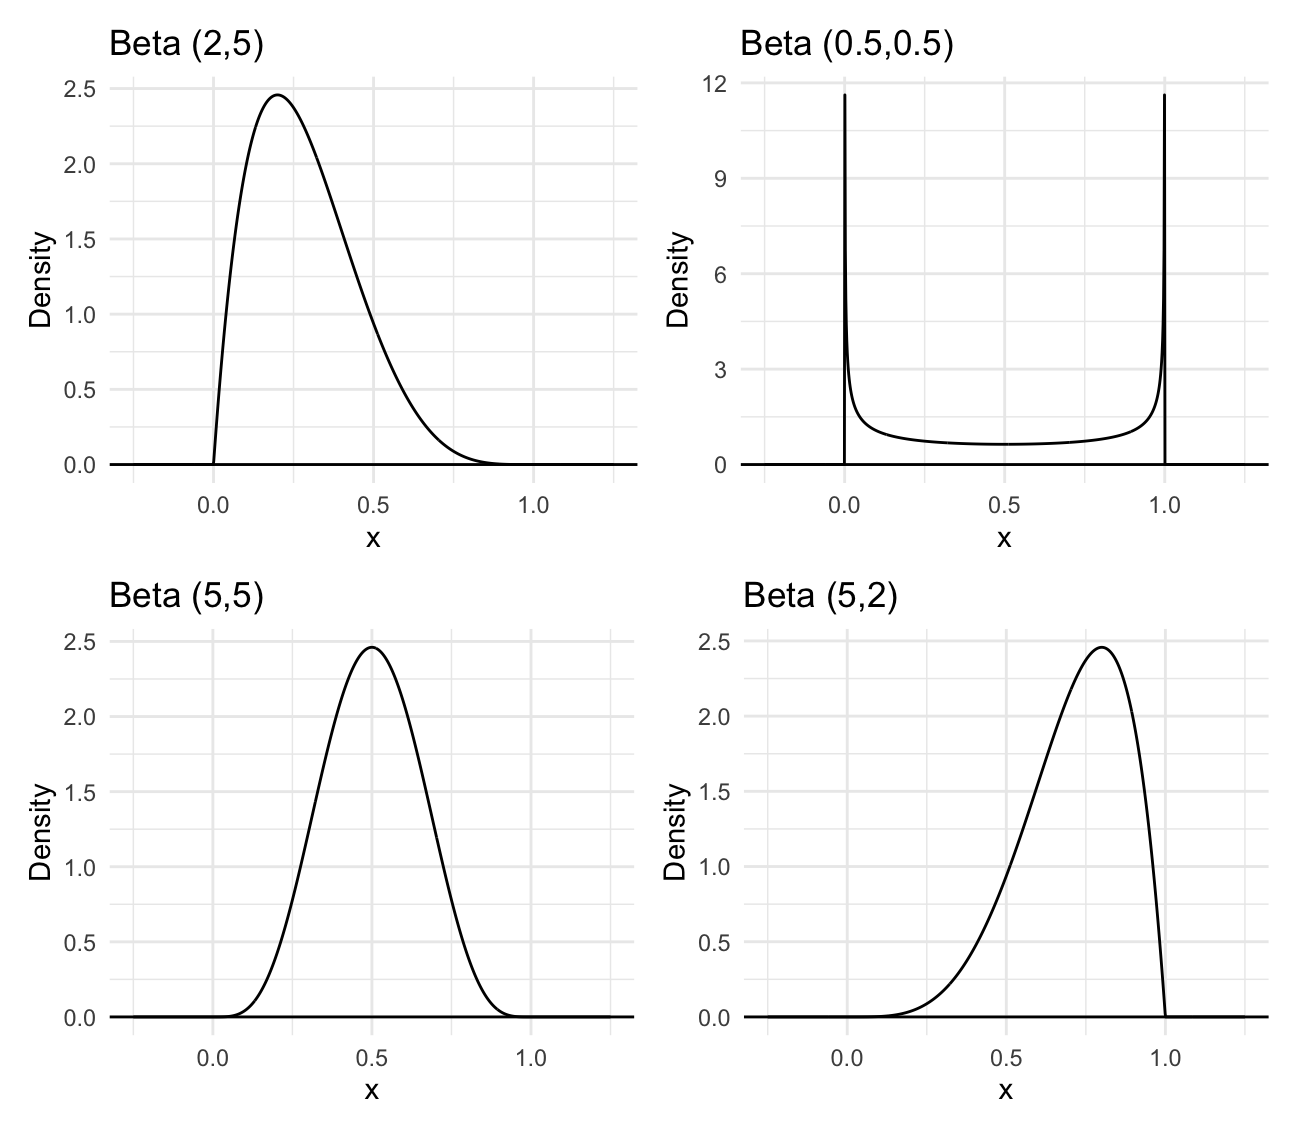
\includegraphics[width=0.47\textwidth]{BDistributions.png}  % Adjust the path and file name
\caption{Beta Distributions Given Different Parameters}
\label{Figure 1}
\end{figure}
This graph and all following graphs were made using \texttt{ggplot2} and organized using \texttt{patchwork} \citep{ggplot} \citep{patchwork}. In these graphs we can see how different each PDF of the distribution can be based on the parameters. Even for something that is completely symmetric it can vary a lot. In the (5,5) distribution it is symmetric and unimodal while the (0.5,0.5) distribution is symmetric but bimodal.
While some probability functions, like the normal curve's, parameters are more meaningful to the sample describing mean and variance, the beta distributions alpha and beta are not as straight forward. The ways to estimate them will be found below however given a sample it is not as simple to find their parameters with something that describes a direct summary statistics of the sample. 

\section{Properties}

One of the most important way of describing a distribution is through sample statistics. Four of the most important sample statistics are the mean, variance, skewness and kurtosis. When discussing these sample statistics it is important to discuss how sample size affects these various statistics. As we can see in Figures \ref{Figure 3} and \ref{Figure 4} below each of the sample statistics approach the population value when the sample size increases. In the first graph we see this for just one sample while in the next we see it for a number of samples showing this reverse megaphone shaped distribution proving that these values approach a certain population value. Another important aspect of sample szie to acknowledge is the large variability that can happen. As we can see with the smaller sample sizes the sample statistics jump all over the place while as it increases it still has some variability but much less. Samples in these graphs were randomly generated samples under the condition that alpha = 2 and beta = 5 using a varying sample size. It is very important to acknowledge these statistics because they give us information like the expected value and how spread apart the data is which is very relevant when thinking about context for real world data following the beta distribution. To compute the skewness and excess kurtosis in these graphs we needed to use the packages \texttt{cumstats} and \texttt{e1071} \citep{cumstats} \citep{e1071}. 





\begin{figure}[H]
\centering
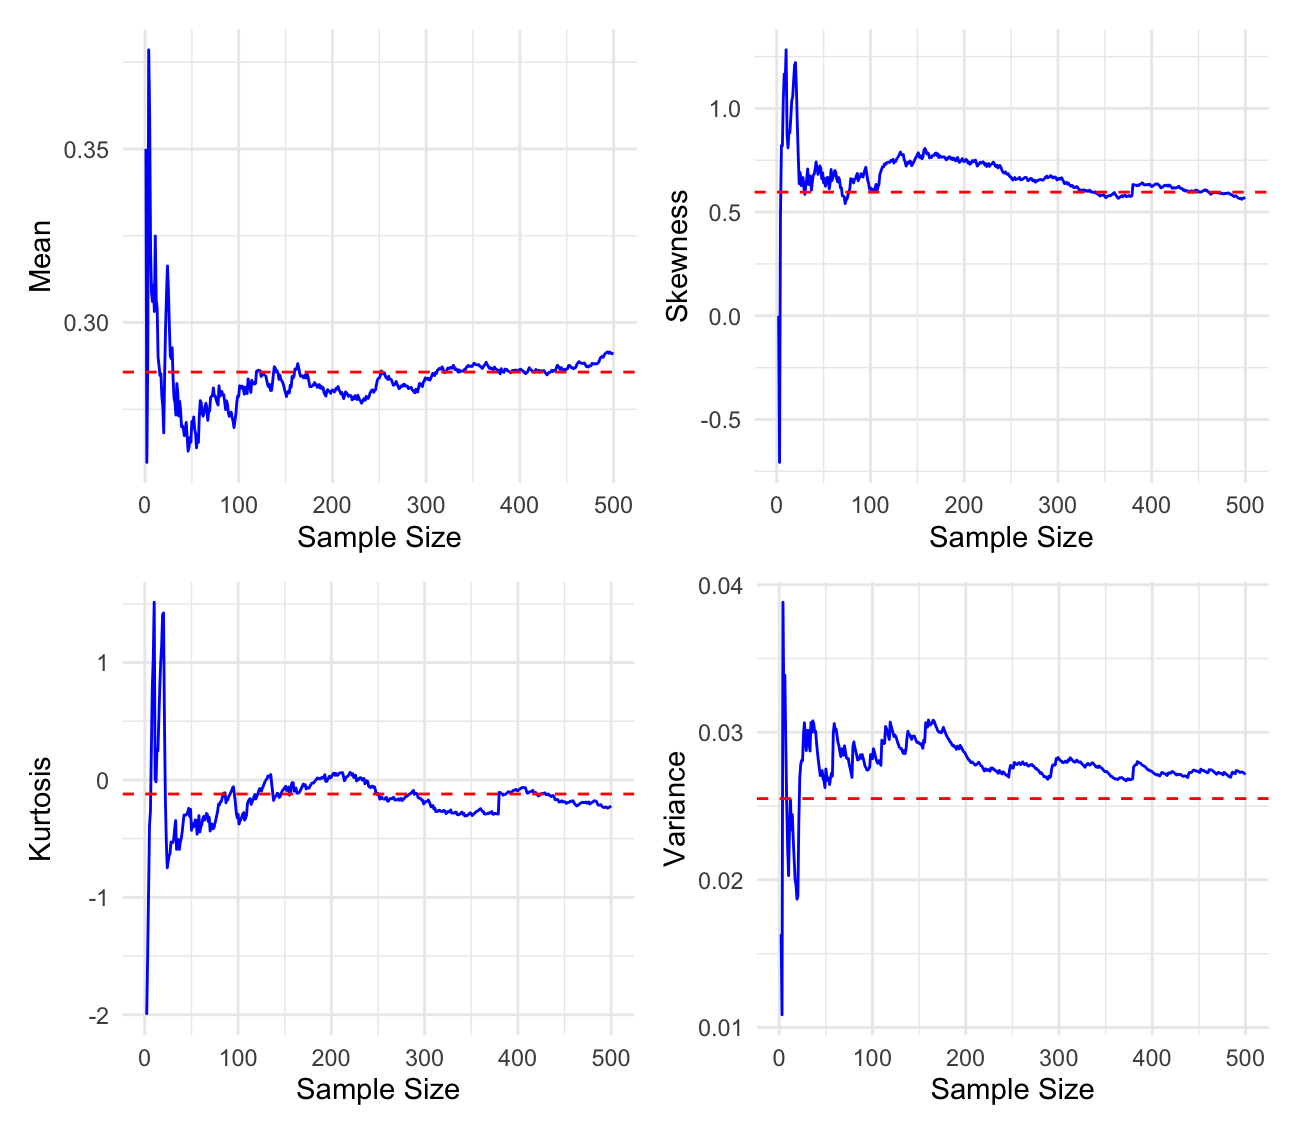
\includegraphics[width=0.47\textwidth]{SampStat}  % Adjust the path and file name
\caption{How Sample Size Effects Summary Stats}
\label{Figure 3}
\end{figure}

\begin{figure}[H]
\centering
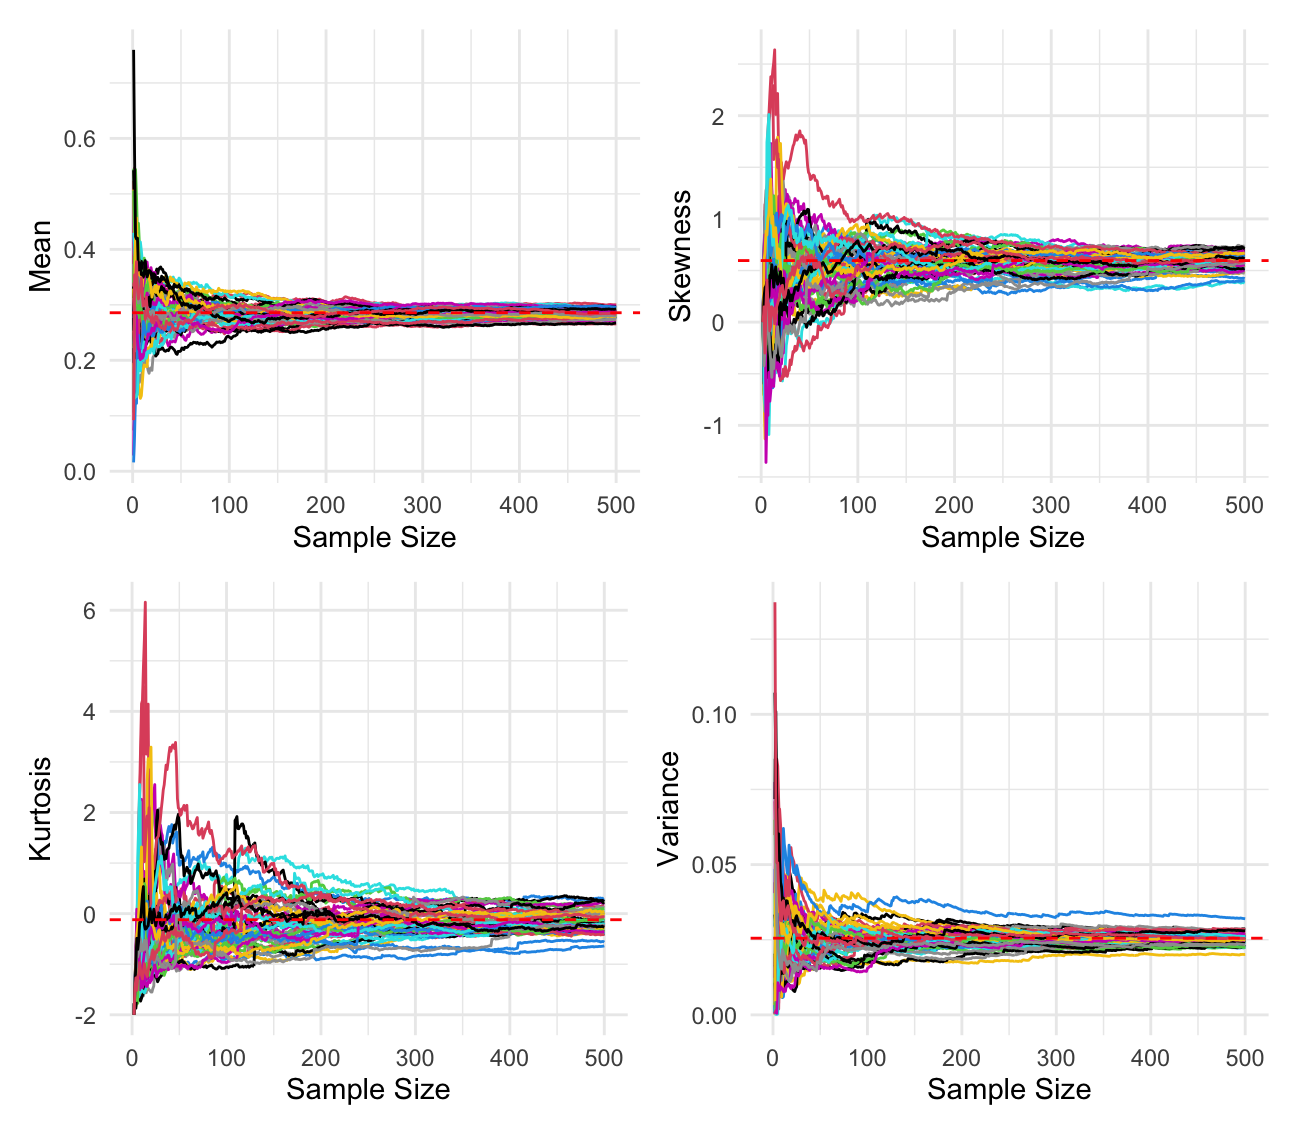
\includegraphics[width=0.47\textwidth]{SimpSampStat}  % Adjust the path and file name
\caption{How Sample Size Effects Summary Stats (Simulated)}
\label{Figure 4}
\end{figure}


Figure \ref{Figure 5} displays a similar concept about these sampling distributions. They all display that the values in the simulation are distributed with a peak at the population value. In other words, they prove that the population value is what it is. For example in the beta 2,5 distribution the mean in each sample when graphed approached 2/7 or 0.2857.



\begin{figure}[H]
\centering
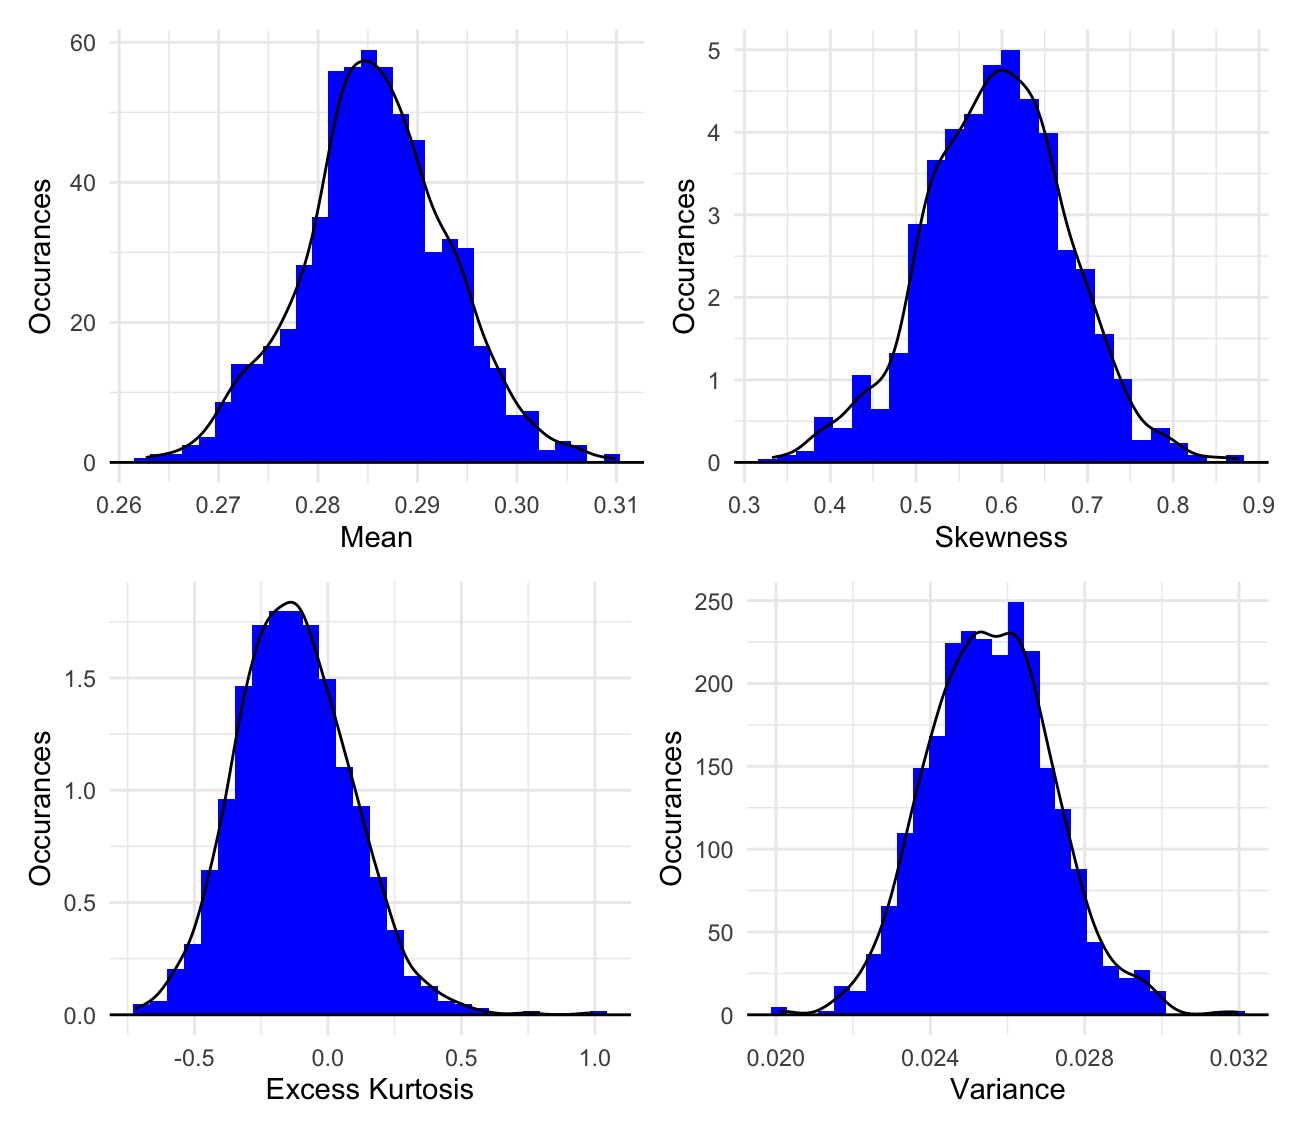
\includegraphics[width=0.47\textwidth]{StatDist}  % Adjust the path and file name
\caption{Sampling Distributions of Summary Statistics}
\label{Figure 5}
\end{figure}

Another important aspect of sample statistics is the way of the finding them. This is different for other probability distributions but there are formulas that can be derived for the beta distribution in closed form. This will give exact statistics about the population of the distribution. However, it is important to be able to estimate these statistics for other distributions so we calculated these computationally as well using moments. Moments use the parameters of the graph and take a region under the curve multiplied by a separate function to estimate a sample statistics like mean. We found each sample statistics using both the formula and in the derived way and this was presented in table \ref{Table 1} in the appendix. 

\section{Estimators}

In order to use the beta distribution we need to be able to estimate the parameters given a sample. There are many ways to do this however two of the most popular are using method of moments and maximum likelihood estimators. The method of moments estimation takes different versions of the sample mean whether it is the mean of the sample itself, the mean of each value squared, the mean of each value cubed, etc. and relates those to the parameters. Since the beta distribution has only two parameters, alpha and beta, we only need two equations to solve. In this case we used the sample mean itself and the mean of each value in the sample squared solving a system of equations. We solved this system using the \texttt{nleqslv} package \citep{nleqslv}. For the maximum likelihood estimator we are trying to optimize a product. While this is very difficult using calculus because of the product rule we took the log of the product to turn it into a sum to make the optimization more simple. We then found the values of alpha and beta that maximize the likelihood function giving the maximum likelihood estimators for the beta distribution. In figure \ref{Figure 7} below we ran a simulation to compute the maximum likelihood estimators and method of moment estimators for 1000 different random samples given the parameters of alpha = 8 and beta = 950. As we can see in the graph they both converge at those two values. However, picking a better estimator is difficult to see within this graph. If we reference table \ref{Table 2} in the appendix however we can clearly see that the maximum likelihood estimators are more precise for both alpha and beta. This is due to the precision being higher, bias being lower and the mean squared estimate being lower. 

\begin{figure}[H]
\centering
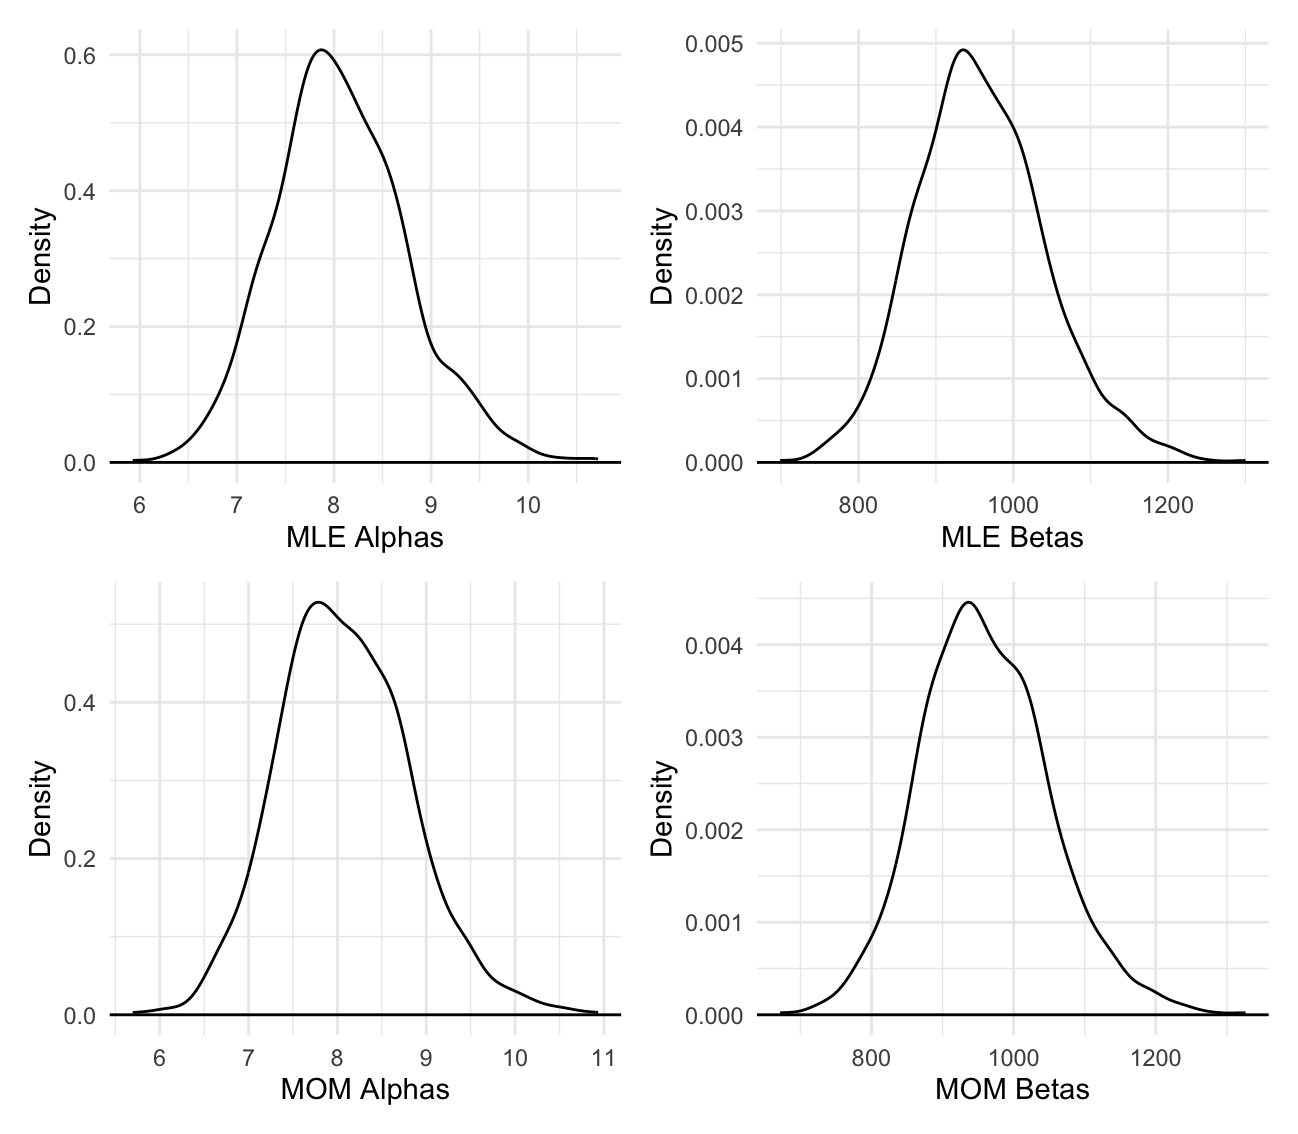
\includegraphics[width=0.47\textwidth]{SimuEsti}  % Adjust the path and file name
\caption{Simulated Estimators for Beta (8,950) Sample}
\label{Figure 7}
\end{figure}

\section{Example}

The most important aspect of the beta distribution is to be able to apply it to real world situations. An example we observed was the proportion of deaths per 1,000 people in many countries around the world. In this sample we computed both the maximum likelihood estimators and method of moment estimators and fit them to the distribution. In Figure \ref{Figure 6} we can see that the MLE and MOM estimators are roughly the same and somewhat accurately describe the distribution. Fitting this sample to a probability distribution will allow us to compute probabilities about the data, simulate future values and is overall very useful. In this particular example we could use the beta distribution to predict the probability of a country having a death rate within a specific range or we could use this data to make assumptions about various regions or groups under a given condition. We were able to organize this data using the \texttt{tidyverse} package \citep{tidyverse}.

\begin{figure}[H]
\centering
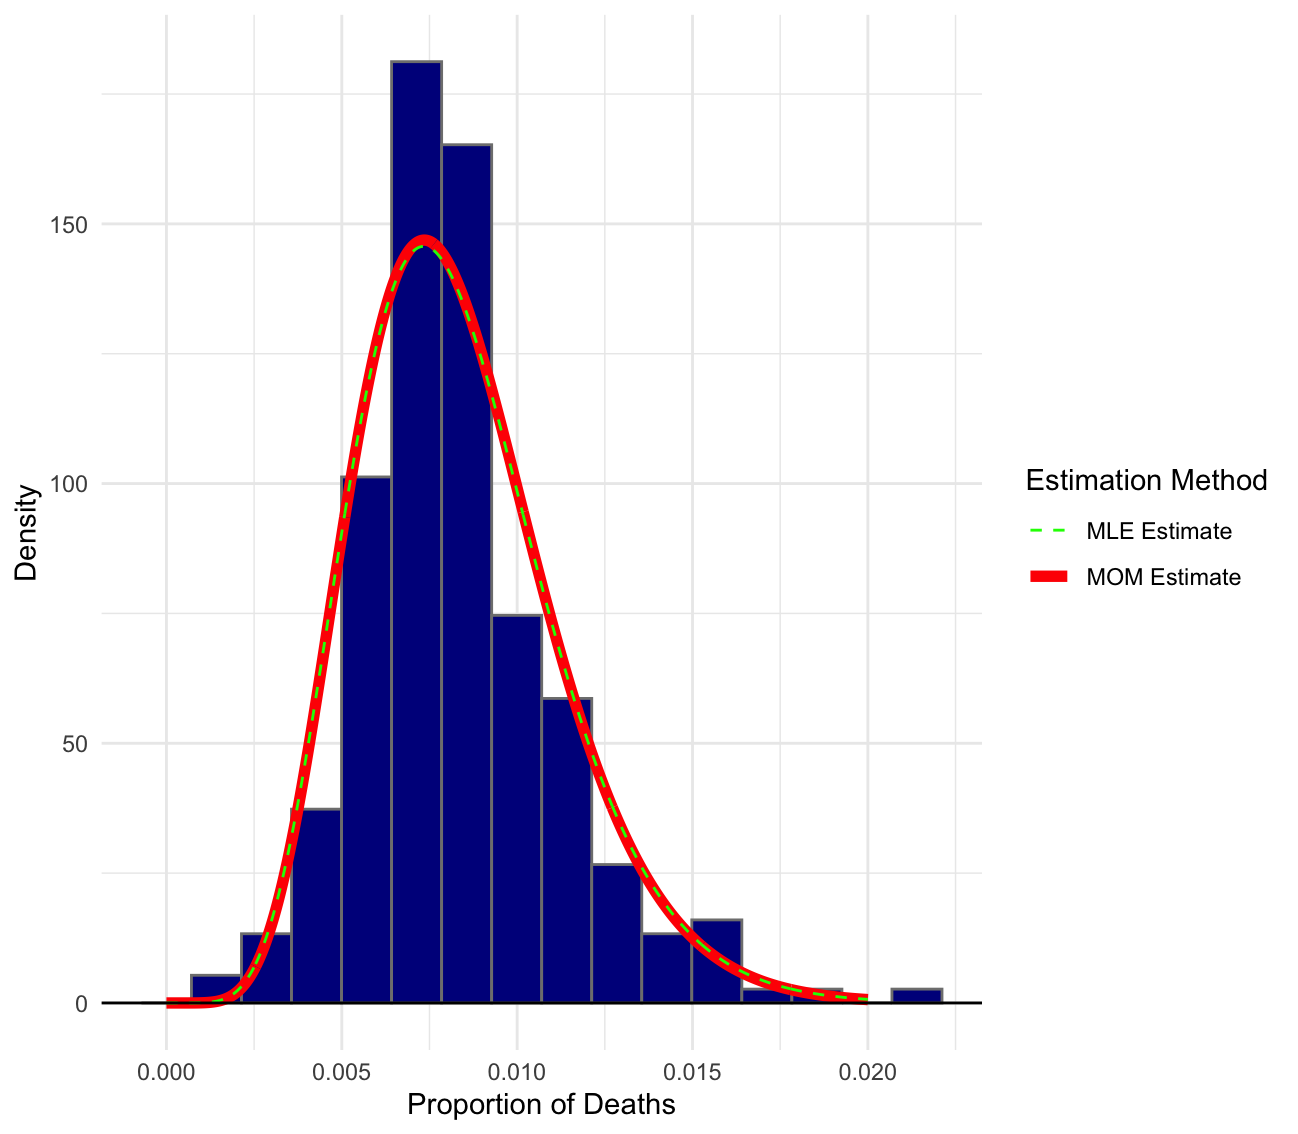
\includegraphics[width=0.47\textwidth]{EstiSamp}  % Adjust the path and file name
\caption{Superimposed Distributions with Estimates on Sample}
\label{Figure 6}
\end{figure}





%%%%%%%%%%%%%%%%%%%%%%%%%%%%%%%%%%%%%%%%%%%%%%%%%%%%%%%%%%%%%%%%%%%%%%%%%%%%%%%%
% Bibliography
%%%%%%%%%%%%%%%%%%%%%%%%%%%%%%%%%%%%%%%%%%%%%%%%%%%%%%%%%%%%%%%%%%%%%%%%%%%%%%%%
\vspace{2em}

\noindent\textbf{Bibliography:} Note that when you add citations to your bib.bib file \emph{and}
you cite them in your document, the bibliography section will automatically populate here.

\begin{tiny}
\bibliography{bib}
\end{tiny}
\end{multicols}

%%%%%%%%%%%%%%%%%%%%%%%%%%%%%%%%%%%%%%%%%%%%%%%%%%%%%%%%%%%%%%%%%%%%%%%%%%%%%%%%
% Appendix
%%%%%%%%%%%%%%%%%%%%%%%%%%%%%%%%%%%%%%%%%%%%%%%%%%%%%%%%%%%%%%%%%%%%%%%%%%%%%%%%
\newpage
\onecolumn
\section{Appendix}


These figures could not fit in the margins of the template above so they have been placed here. Each graph was created using \texttt{ggplot2} and organized using \texttt{patchwork} \citep{ggplot} \citep{patchwork}. Each table was made using \texttt{xtable} \citep{xtable}. 

This graph displays how the population distribution for various beta PDF's describe a random sample generated given the parameters. As we can see the PDF generally follows the density graph for the histogram displaying that large samples described given various parameters replicate the population distribution somewhat well. 

\begin{figure}[H]
\centering
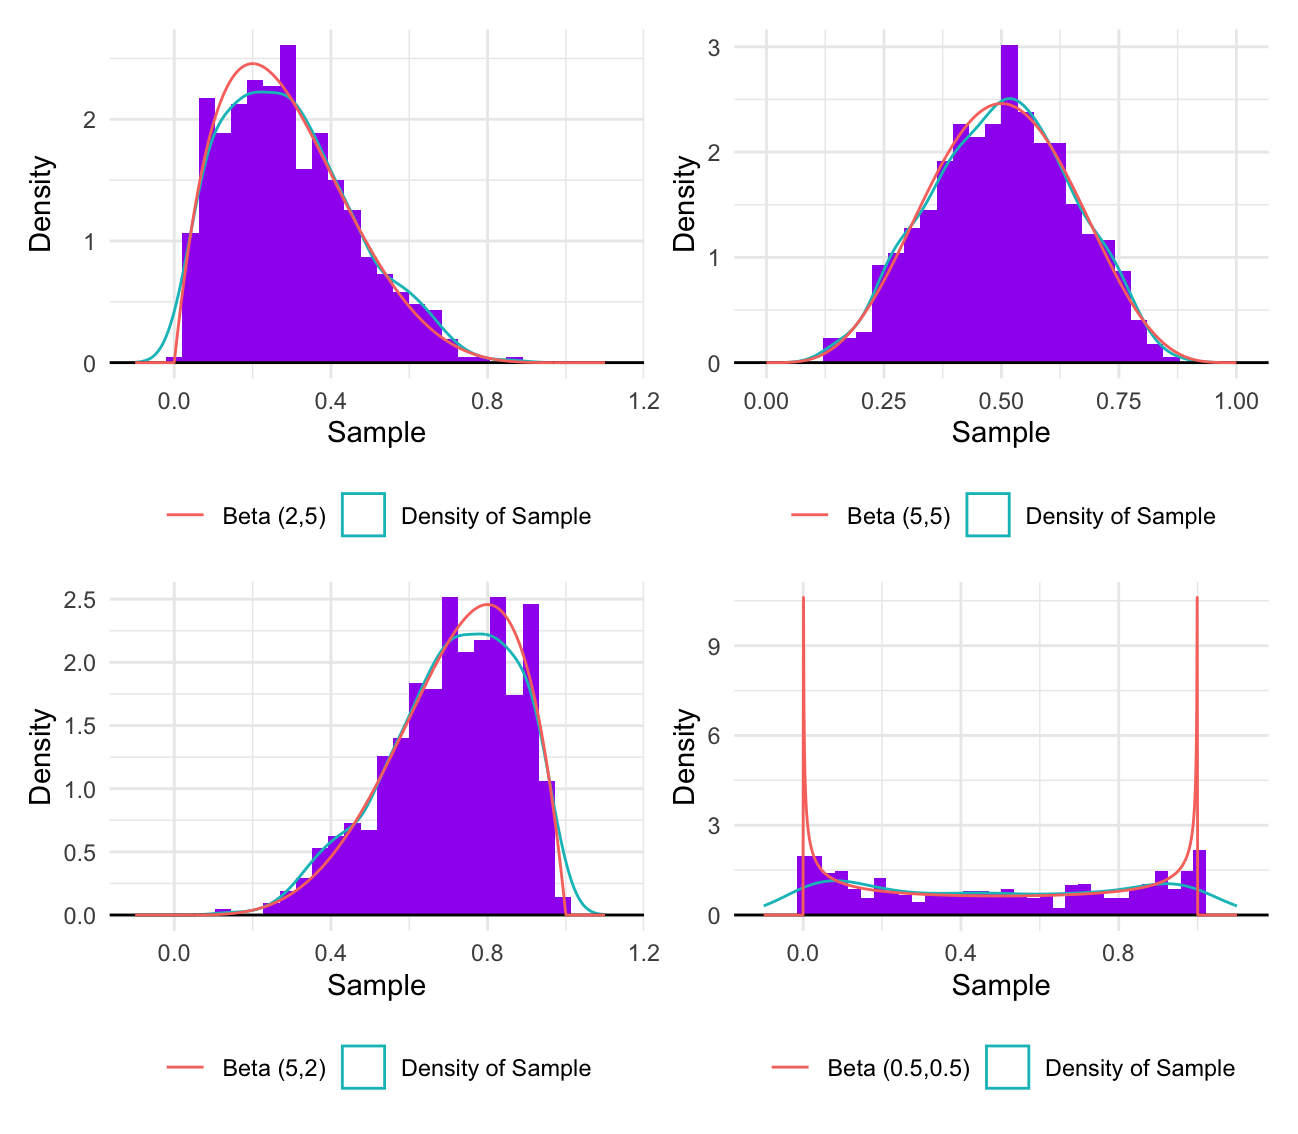
\includegraphics[width=0.47\textwidth]{SampDist}  % Adjust the path and file name
\caption{Samples of Beta Distributions}
\label{Figure 2}
\end{figure}

\begin{table}[ht]
\centering
\begin{tabular}{rrrrrrrl}
\hline
& Alpha & Beta & Mean & Variance & Skewness & Excess Kurtosis & Method \\ 
\hline
1 & 2.00 & 5.00 & 0.29 & 0.03 & 0.60 & -0.12 & Formula \\ 
2 & 5.00 & 5.00 & 0.50 & 0.02 & 0.00 & -0.46 & Formula \\ 
3 & 5.00 & 2.00 & 0.71 & 0.03 & -0.60 & -0.12 & Formula \\ 
4 & 0.50 & 0.50 & 0.50 & 0.12 & 0.00 & -1.50 & Formula \\ 
5 & 2.00 & 5.00 & 0.29 & 0.03 & 0.60 & -0.12 & Derived \\ 
6 & 5.00 & 5.00 & 0.50 & 0.02 & -0.00 & -0.46 & Derived \\ 
7 & 5.00 & 2.00 & 0.71 & 0.03 & -0.60 & -0.12 & Derived \\ 
8 & 0.50 & 0.50 & 0.50 & 0.12 & -0.00 & -1.50 & Derived \\ 
\hline
\end{tabular}
\caption{Summary Statistics Using Different Methods for the Beta Dist.}
\label{Table 1}
\end{table}


\begin{table}[ht]
\centering
\begin{tabular}{rlrrr}
  \hline
 & Names & Bias & Precision & MSE \\ 
  \hline
1 & Alpha MLE & 0.0720 & 2.1269 & 0.4754 \\ 
  2 & Alpha MOM & 0.0822 & 1.8286 & 0.5536 \\ 
  3 & Beta MLE & 9.1142 & 0.0001 & 7134.5577 \\ 
  4 & Beta MOM & 10.3424 & 0.0001 & 8290.0516 \\ 
   \hline
\end{tabular}
\caption{Predictors to determine how good our estimators are}
\label{Table 2}
\end{table}


\end{document}
